\documentclass[12pt]{article}
\usepackage{graphicx}
\usepackage{fullpage}
\usepackage{verbatim}
\usepackage{caption}
\usepackage{float}
\usepackage[nottoc]{tocbibind} 
\usepackage{appendix}
\usepackage{titlesec}
\usepackage{tikz}
\usepackage{listings}
\usepackage{hyperref}
\hypersetup{
    colorlinks=true,
    linkcolor=blue,
    filecolor=magenta,      
    urlcolor=blue,
}
\usepackage[utf8]{inputenc}
\urlstyle{same}
\usetikzlibrary{shapes,arrows}
\titleformat{\chapter}[display]
  {\normalfont\bfseries}{}{0pt}{\Large}
  \usepackage[T1]{fontenc}
\usepackage[utf8]{inputenc}

  


\begin{document}
  \begin{titlepage}
    \begin{center}
      \begin{Large}
      \textbf{ Assignment- 13\\
       \vspace*{0.5cm}
       ELP - 718 Telecom Software Laboratory\\
       \vspace{1cm}
       Ch Krishna Chaitanya\\
       2019JTM2674\\
       2019-21\\}
      \end{Large}
       \vspace{1cm}
      {\Large  A report on Socket Programming using C}
       \vfill
       \begin{figure}[h!]
          \centering
          
\includegraphics{iitdelhi.png}
       \end{figure}
       \vfill
      \begin{Large}
      \textbf{ Bharti School of \\
       Telecommunication Technology and Management\\
       IIT Delhi\\
       India\\
      }\end{Large}
       \medskip
       \today
    \end{center}
    \vfill
  \end{titlepage}
  
  \tableofcontents
  
  \clearpage
  \section*{Objective Statement}
   To test our understanding on Socket programming using C.

  \section{Problem Statement -1}
 To Create a server that is capable of handling multiple clients using TCP communication sockets
 
  \subsection{Problem Satement}
  
  \subsection{Algorithm and Implementation}
  \begin{itemize}
  \item Create File with username and password
  \item Create a Server capable of connecting to multiple clients
  \item Validate User from Client Side
  \item After finishing chat, ask for mobile number to send messages to particular mobile number
  \item If user is not present store it in a file
  \item After availability of user, send the stored chat
  \item Delete the file after sending chat information.

  \end{itemize}
  
  \subsection{Flowchart}
    % Define block styles
\tikzstyle{decision} = [diamond, draw, fill=blue!20, 
    text width=4.5em, text badly centered, node distance=3cm, inner sep=0pt]
\tikzstyle{block} = [rectangle, draw, fill=blue!20, 
    text width=6.5em, text centered, rounded corners, minimum height=3em]
\tikzstyle{line} = [draw, -latex']
\tikzstyle{cloud} = [draw, ellipse,fill=red!20, node distance=3cm,
    minimum height=3em]
\begin{center}    
\begin{tikzpicture}[node distance = 2cm, auto]
    % Place nodes
    
    \node [cloud] (init) {start};
    \node [block, below of=init] (First) {Establish Client server Connection};
    \node [block, below of=First] (Second) {Client Enter Usernmae and Password};
    \node [decision, below of=Second] (Third) {If Valid User?};
    \node [block, left of=Third,node distance=3cm] (Eigth) {Invalid User};
     \node [block, below of=Third,node distance=3cm] (Fouth) {Chat};
     \node [decision, below of=Fouth,node distance=3cm] (Fifth) {If Exit?};
     
    \node [block, below of=Fifth,node distance=3cm] (Seventh) {Send Data to given Mobile No.};
    \node [block, left of=Fifth,node distance=3cm] (Sixth) {Continue};
    \node [cloud, below of=Seventh] (last_1) {stop};
  
    
    % Draw edges
    \path [line] (init) -- (First);
    \path [line] (First) -- (Second);
    \path [line] (Second) -- (Third);
     \path [line] (Third) -- node {yes}(Fouth);
     \path [line] (Fouth) --(Fifth);
     \path [line] (Fifth) --(Sixth);
     \path [line] (Sixth) |-(Fouth);
     \path [line] (Third) -- node{no}(Eigth);
     \path [line] (Eigth) |-(Second);
     \path [line] (Fifth) --(Seventh);
     \path [line] (Seventh) --(last_1);

     
    
   
\end{tikzpicture}
\end{center}
  
 \newpage
  \subsection{Test Cases}
  
	\subsubsection{Input}
	Enter User name\\
Enter Password\\
\subsubsection{Output}
start Chat
\subsection{Screenshots}
\subsubsection{Screenshot1}
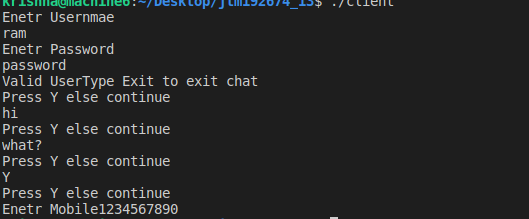
\includegraphics[width=\linewidth]{lab13_c.png}
\clearpage
\newpage
\section{Problem Statement -2}
 To Create a normalised score rating application.
 
  \subsection{Problem Satement}
  
  \subsection{Algorithm and Implementation}
  \begin{itemize}
  \item Create File with name and other information
  \item Input File Name
  \item Send file data from client side to server side
  \item On server side, assign the rating as given
  \item Calculate Normalised Percentage
  \item Send it to client
  \item Display Information
  \end{itemize}
  
  \subsection{Flowchart}
    % Define block styles
  \tikzstyle{decision} = [diamond, draw, fill=blue!20, 
    text width=4.5em, text badly centered, node distance=3cm, inner sep=0pt]
\tikzstyle{block} = [rectangle, draw, fill=blue!20, 
    text width=5em, text centered, rounded corners, minimum height=4.5em,node distance=2.3cm]
\tikzstyle{line} = [draw, -latex']
\tikzstyle{cloud} = [draw, ellipse,fill=red!20, node distance=2.5cm,
    minimum height=3em]
  \begin{center}    
\begin{tikzpicture}[node distance = 2cm, auto]
    % Place nodes
    
     \node [cloud] (init) {start};
    \node [block, below of=init] (First) {Create File};
    \node [block, below of=First] (Second) {Enter File name};
    \node [block, below of=Second] (Third) {Transfer File to Server};
    \node [block, below of=Third] (Fourth) {Calculate Normalised Score};
    \node [block, below of=Fourth] (Fifth) {Send Normalised Score to Client};
    \node [block, below of=Fifth] (Sixth) {Display Data};
    \node [cloud, below of=Sixth] (Seventh) {Stop};
    
    
    % Draw edges
    \path [line] (init) -- (First);
    \path [line] (First) -- (Second);
    \path [line] (Second) -- (Third);
     \path [line] (Third) -- (Fourth);
    \path [line] (Fourth) -- (Fifth);
    \path [line] (Fifth) -- (Sixth);
    \path [line] (Sixth) -- (Seventh);
  
   
    
\end{tikzpicture}
\end{center}
    \subsection{Test Cases}
  
	\subsubsection{Input}
	Enter File Nmae\\
file1.txt\\
\subsubsection{Output}
Hey Prerna Singh, your normalised score is 0.848485
\subsection{Screenshots}
\subsubsection{Screenshot1}

\includegraphics[width=\linewidth]{lab13_a.png}
\subsubsection{Screenshot2}

\includegraphics[width=\linewidth]{lab13_b.png}
\clearpage
\newpage
 \appendix
   \appendixpage
   \addappheadtotoc
  \section*{Problem 1}
  {\large \textbf{code:}}
  \verbatiminput{ps1_server.c}
  \section*{Problem 2}
  {\large \textbf{Server code:}}
  \verbatiminput{ps2_server.c}
  {\large \textbf{Client code:}}
  \verbatiminput{ps2_client.c}
  
\newpage
\begin{thebibliography}{11}
\bibitem{flowchart} 
Flowchart using Latex\\
Kjell Magne Fauske \\
\url{http://www.texample.net/tikz/examples/simple-flow-chart/}

\bibitem{Socket Programming}
Socket Programming \\
\url{https://www.geeksforgeeks.org/socket-programming-cc/}

\bibitem{Socket Tutorial}
Socket Tutorial\\
\url{http://www.linuxhowtos.org/C_C++/socket.htm}

\bibitem{Network Programming}
Network Programming\\
\url{https://beej.us/guide/bgnet/}

\bibitem{Sockets Tutorial}
Sockets Tutorial\\
\url{https://www.cs.rpi.edu/~moorthy/Courses/os98/Pgms/socket.html}

\end{thebibliography}

   
   
\end{document}
